\section{Summary of Papers}
\label{sec:summary}

\subsection{AutoNER}
AutoNER \cite{autoner} has two contributions: Fuzzy LSTM CRF and Tie-or-Break scheme.
\\

\noindent\textbf{Fuzzy LSTM CRF}
Have to read about CRF and why they work.
\\

They also introduce a training mechanism which models the noise in supervision. 
\noindent\textbf{Tie-or-Break Scheme}
\\

\begin{figure*}[h!]
	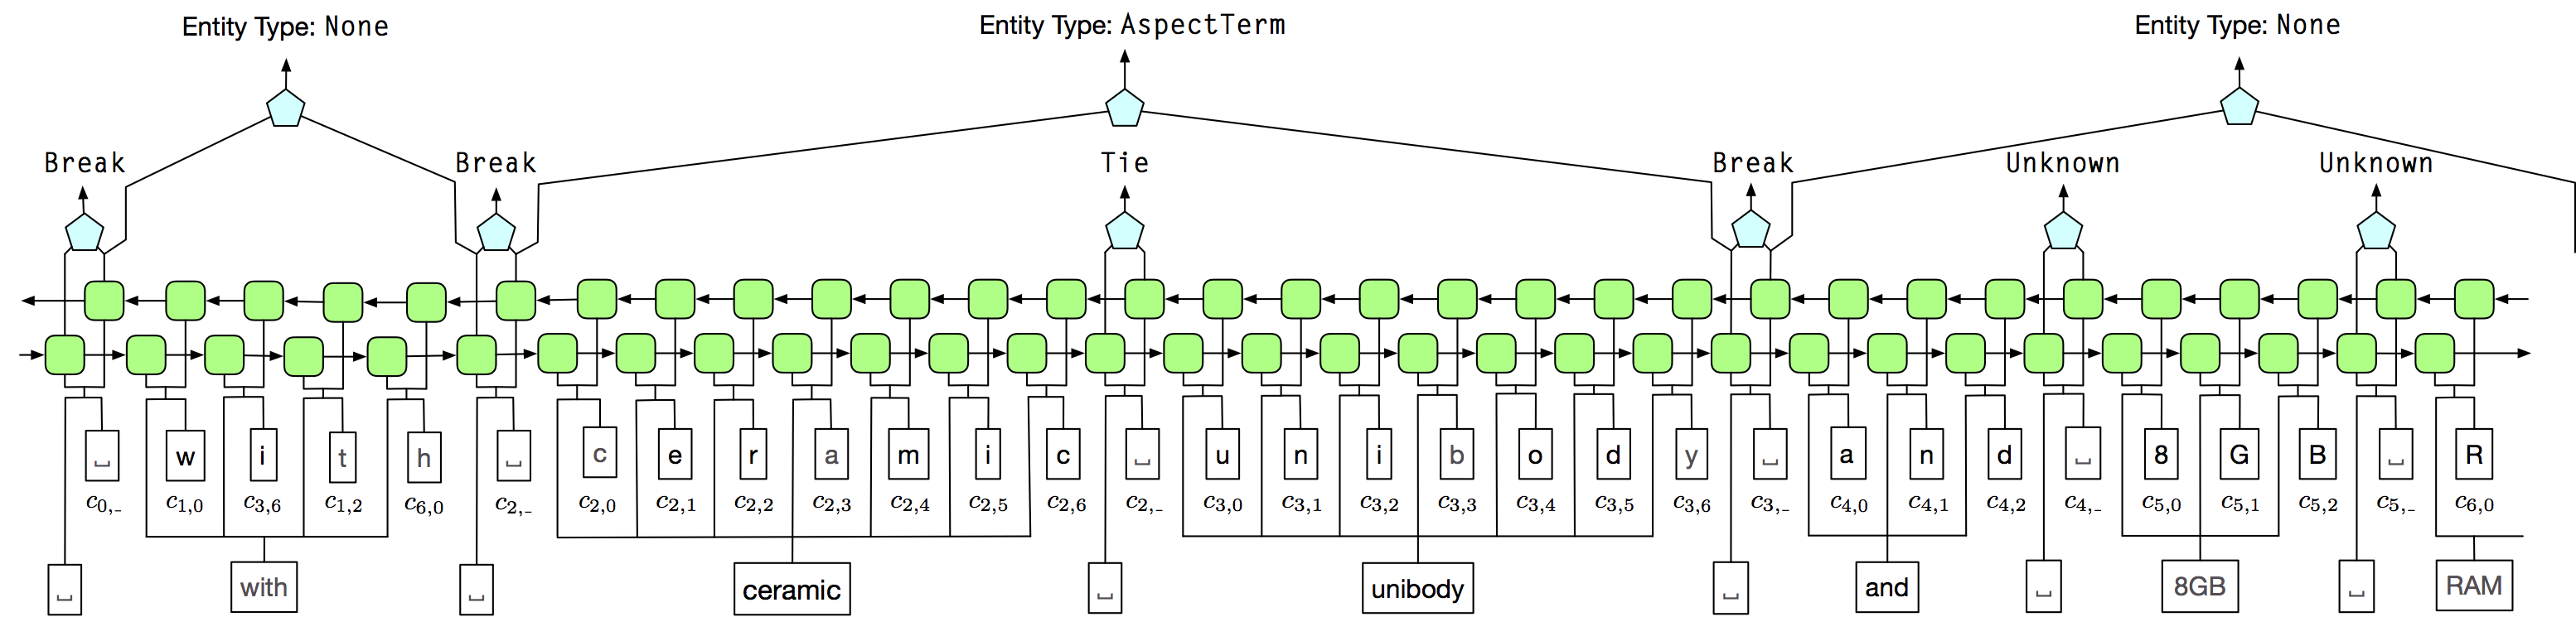
\includegraphics[scale=0.3]{images/autoner_tie_or_break.png}
	\caption{\label{fig:tie_or_break}Overview of the Tie-or-Break scheme used in AutoNER.}
\end{figure*}

